\documentclass[border=12pt]{standalone}
\usepackage{tikz}
\usetikzlibrary{shapes.geometric, arrows.meta, positioning, calc, fit, backgrounds}
\usepackage{fontspec}
\usepackage{amsmath,amssymb}
\setmainfont{DejaVu Sans}

\begin{document}
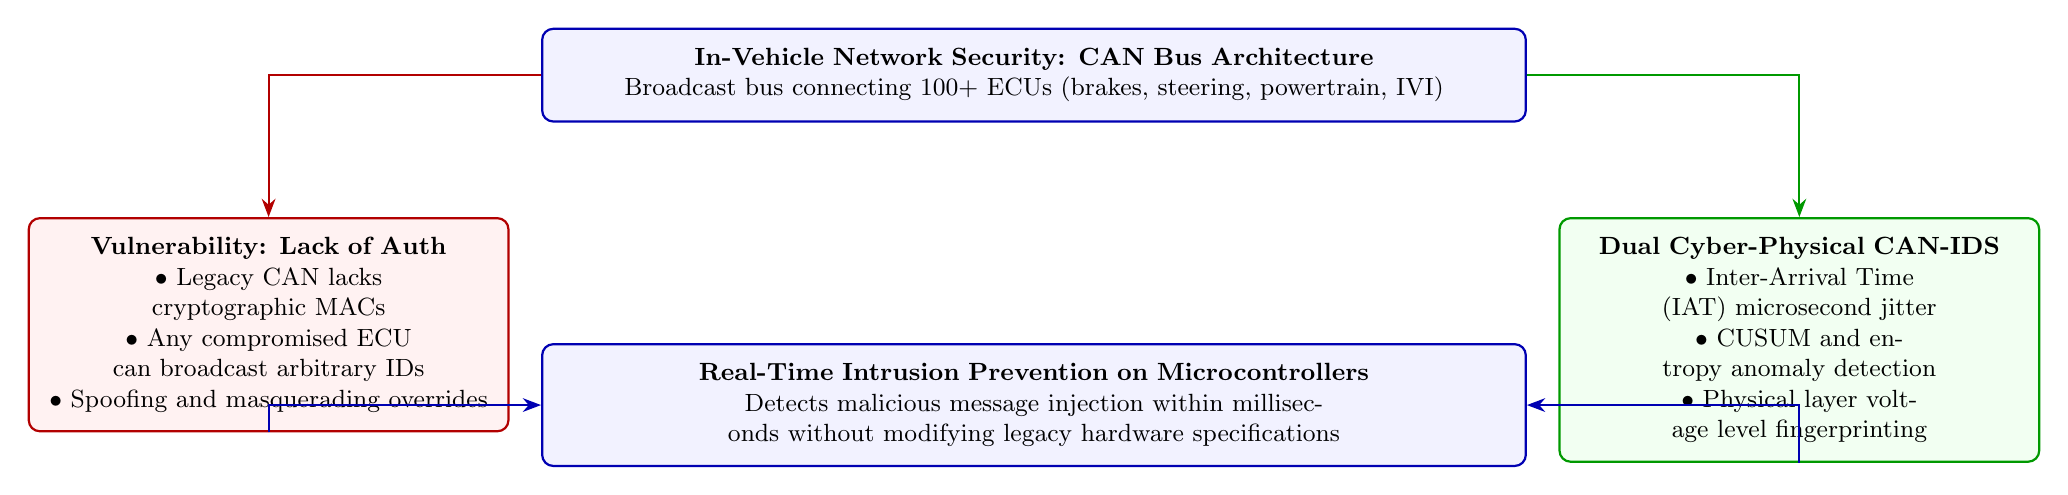
\begin{tikzpicture}[
    font=\small,
    >=Stealth,
    node distance=1.2cm,
    block/.style={rectangle, draw=blue!70!black, fill=blue!5, rounded corners=4pt, thick, align=center, inner sep=7pt},
    alertblock/.style={rectangle, draw=red!70!black, fill=red!5, rounded corners=4pt, thick, align=center, inner sep=7pt},
    greenblock/.style={rectangle, draw=green!60!black, fill=green!5, rounded corners=4pt, thick, align=center, inner sep=7pt},
    amberblock/.style={rectangle, draw=orange!80!black, fill=orange!5, rounded corners=4pt, thick, align=center, inner sep=7pt}
]

\node[block, text width=12cm] (top) {\textbf{In-Vehicle Network Security: CAN Bus Architecture}\\Broadcast bus connecting 100+ ECUs (brakes, steering, powertrain, IVI)};

\node[alertblock, below left=1.2cm and 0.4cm of top, text width=5.6cm] (threat) {\textbf{Vulnerability: Lack of Auth}\\$\bullet$ Legacy CAN lacks cryptographic MACs\\$\bullet$ Any compromised ECU can broadcast arbitrary IDs\\$\bullet$ Spoofing and masquerading overrides};

\node[greenblock, below right=1.2cm and 0.4cm of top, text width=5.6cm] (ids) {\textbf{Dual Cyber-Physical CAN-IDS}\\$\bullet$ Inter-Arrival Time (IAT) microsecond jitter\\$\bullet$ CUSUM and entropy anomaly detection\\$\bullet$ Physical layer voltage level fingerprinting};

\node[block, below=2.8cm of top, text width=12cm] (bottom) {\textbf{Real-Time Intrusion Prevention on Microcontrollers}\\Detects malicious message injection within milliseconds without modifying legacy hardware specifications};

\draw[->, thick, red!70!black] (top) -| (threat);
\draw[->, thick, green!60!black] (top) -| (ids);
\draw[->, thick, blue!70!black] (threat) |- (bottom);
\draw[->, thick, blue!70!black] (ids) |- (bottom);

\end{tikzpicture}
\end{document}
